%--------------------------------------------------------------------------
%
%                                                    SOLUTION
%
%--------------------------------------------------------------------------

\begin{center}
\vspace*{5mm}
\noindent {\Large {\bf Le manège à plancher rétractable }}
\end{center}

\begin{enumerate}
\item Le manège est en rotation, le référentiel associé n'est donc pas d'inertie (galiléen). Si ($Oxyz$) est le repère associé au référentiel de l'observateur hors manège, on nomme ($Ox'y'z$) le repère tournant associé au manège, avec l'axe $Ox'$ partant du centre du manège et passant par (le centre de gravité de) la personne et $Oy'$ tel que le repère soit direct (on rappelle que $z = z'$).

\begin{minipage}{0.5\textwidth}Les forces s'appliquant sur la personne sont :
\begin{itemize}
\item son poids $\vec{P}=m\vec{g}=-mg\hat{e}_z =-mg\hat{e}_{z'}$
\item la force de liaison de la paroi, $\vec{N} =N_x\hat{e}_{x'}$
\item la force de frottement statique avec la paroi $\vec{T} = T_z\hat{e}_{z'}$
\item la force centrifuge $\vec{f}_{\rm cent.} = -m\vec\omega\wedge (\vec\omega\wedge\overrightarrow{OG}) = mR\omega^2\hat{e}_{x'}$
\item les autres forces d'inertie sont nulles.
\end{itemize}
Pour que l'équilibre ait lieu, la somme de ces forces doit être nulle. Il en ressort que la force de réaction de la paroi doit compenser la force centrifuge, $N_x = -mR\omega^2$, et que la force de frottement statique doit compenser le poids, $T_z = mg$.
On voit donc en particulier qu'on ne peut s'affranchir du frottement statique dans la description du problème.
\end{minipage}\hspace*{5mm}
\begin{minipage}{0.5\textwidth}
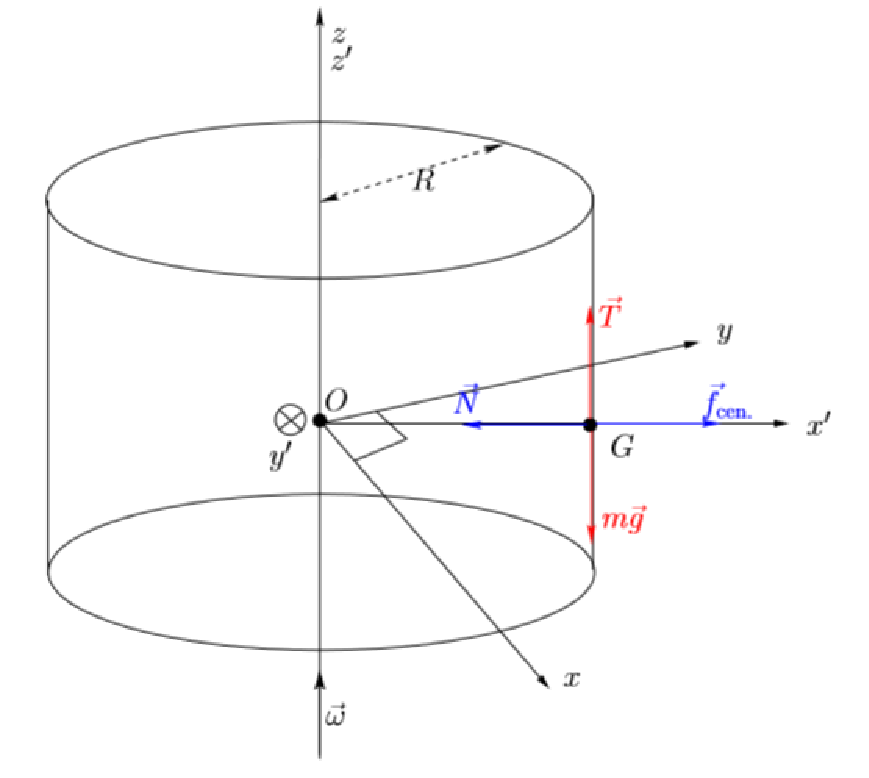
\includegraphics[width=7cm]{figures/serie14_c_fig1.pdf}
\end{minipage}
\item On sait d'après les lois de Coulomb sur le frottement statique que la condition de non glissement de la personne le long de la paroi est $|T_z| \leq \mu |N_x|$.
En utilisant les conditions d'équilibre de la question a), on en déduit que :
\begin{equation}\omega^2 \geq \frac{g}{\mu R},\end{equation}c'est à dire \begin{equation}\omega \geq\omega_{\rm min}\quad\rm{avec}\quad\omega_{\rm min} = \sqrt{\frac{g}{\mu R}}.\end{equation}
\end{enumerate}